\chapter{A Tutorial Game}
\label{ch:tutorial_game}
As the second part of my own work, I designed and implemented a prototype for an educational game for \gls{uml} activities in the context of Reactive Blocks, nicknamed simply \emph{The Reactive Blocks game}. Based on the tutorial described in Ch.~\ref{ch:reactive_blocks_tutorial}, this game teaches the same concepts in similar ways, but in a different environment. This chapter covers the motivation for creating the game, as well as a description of the design and implementation of the prototype. Additionally, a user test was conducted in an effort to uncover usability issues with the game prototype, supporting an evaluation of the game prototype.

\section{Motivation}
\label{sec:game_motivation}
\emph{Game-based learning} is a concept that is becoming more and more popular. Sections~\ref{sec:game_based_learning} and~\ref{sec:learning_with_games} describe how and why this approach to learning is becoming popular, with examples of some more or less successful learning games, and it is clear that games can successfully be used to teach various subjects and concepts.

\noindent
Given the success of other educational games, it may be interesting to see if we can create a good game for learning \gls{uml} activities, perhaps in the context of Reactive Blocks, in order to increase student motivation and understanding of how \gls{uml} modeling works. In Sect.~\ref{sec:tutorial_test_results}, we saw that most of the test subjects that provided feedback answered that they might prefer learning about \gls{uml} activities through a game than a tutorial, so there could be a real interest for a game like this, given that it is well-designed.

\subsection{Goals}
\label{sec:game_goals}
Like with the tutorial in Ch.~\ref{ch:reactive_blocks_tutorial}, I initially set some goals for the design and implementation of the game. These goals are primarily based on experiences from the tutorial implementation and test, as well as the good practices from Sect.~\ref{sec:good_practices_games}.

\paragraph{Immersion} The primary goal for the game is to provide an environment where players can immerse themselves in the learning experience. This involves giving the players a sense of identity within the game, and providing them with challenges that are easily visualized and comprehended within the given environment.

\paragraph{Exploration and Guidance} \gls{uml} activities can be used to model very complex systems, and learning how to do this is not a trivial process. The game is thus likely to benefit from providing some guidance to players, as opposed to complete freedom to explore~\cite{andersen:tutorials_impact}. Some freedom is still necessary, to facilitate creativity and deeper learning~\cite{bonawitz:double_edged_pedagogy}. The goal is then that the game should be primarily focused around a tutorial-like guided path for learning about concepts within \gls{uml} activities, but with the possibility for players to find their own solutions to problems. Players should also be encouraged to explore other perspectives, and maybe find different or even \emph{better} solutions to the same problems.

\paragraph{Level of Difficulty} The target audience for the game is the same as for the tutorial (Sect.~\ref{sec:target_audience}). The game should be easy enough for less knowledgeable users to get started without frustration, but eventually provide challenges that feel relevant also to the more experienced. Players should also have the option to skip challenges they feel are less relevant to them, or that involve concepts they have already mastered, in order to avoid the game experience becoming tedious.

\paragraph{Lessons from the Tutorial} The design and implementation of the tutorial in Ch.~\ref{ch:reactive_blocks_tutorial} fulfilled some, but not all of the goals that were set. The approach seemed to provide a decent learning experience, but with some potential for improvement. A goal for the game is to build on the parts of the tutorial that were successful, such as the teaching order, and additionally include some of the parts that were not implemented or successful, such as having everything in one place. Since the game still will be based on Reactive Blocks, many of the same challenges will be present, but with a game, there should be more options for providing resources within the same platform, such as help-on-demand.

\section{Game Design}
\label{sec:game_design}
When developing the concept of the game, a few points were considered. First of all, it should involve some sort of main character, giving the player a sense of identity. Secondly, the game concept must accommodate a range of different types of challenge that are suited for learning about concepts like concurrency, modularization and reuse. Finally, the concept must be relatively easy to prototype, as the available time to implement the game was fairly limited.

\subsection{The Final Concept}
\label{sec:game_final_concept}
With the above design points in mind, I settled on a two-dimensional maze-navigating game, where the player controls a character or set of characters through operations and logic in Reactive Blocks. The main character, Malcolm, must perform one or more goals to complete the level, such as gathering stars. In order to get to these stars however, Malcolm must perform some other tasks, such as gathering keys, or invoke the assistance of other characters in the game.

\noindent
This concept was chosen for the following reasons:
\begin{itemize}
	\item Two-dimensional games are quick and easy to implement, both graphically and programming-wise, given an appropriate framework.
	\item Since the purpose of the game is to teach \gls{uml} activities, it makes most sense to provide a game environment where the player must program their characters' path in advance, and then see if they modeled the desired behavior correctly. A two-dimensional maze-navigating game makes it easy for players to get a clear overview of what they are supposed to do.
	\item Despite being relatively simple to implement, a two-dimensional maze-game offers a lot of possibilities in the form of obstacles and challenges the player must overcome in order to complete each level.
\end{itemize}

\noindent
Even with such a flexible concept in place, it was no trivial task to create levels and challenges that let the user learn about \gls{uml} activity concepts in an intuitive and reasonable way. In addition, I had to consider how each concept should be introduced within its level, so that the user would know what to expect.

\subsection{The Tutorial Part}
\label{sec:game_tutorial}
One of the most important goals for the game was to provide an environment where the player could find all the information needed to complete a level, instead of having to switch between contexts or search through external sources. Players would be creating the logic for each level in Reactive Blocks, generate code from these models, and run it to see if it was correct. Thus, additional information, such as concept introductions, level maps, and help-on-demand, had to be presented inside Reactive Blocks. Unfortunately, because I was unable to alter the Reactive Blocks environment, I could still not provide a tutorial mode, just as with the tutorial in Ch.~\ref{ch:reactive_blocks_tutorial}.

\noindent
Instead of a tutorial mode in Reactive Blocks, a different solution presented itself. I could create a separate program with a window that would contain the most basic information needed for each level, with internal links to additional resources. This would of course not be completely within the context of Reactive Blocks, but hopefully a decent substitute for the lack of a real tutorial mode.

\noindent
Designing the tutorial window presented some challenges of its own. The window needed to be small enough for players to be able to keep it on their screen together with the Eclipse/Reactive Blocks window, preferably also for smaller screens like on laptops. At the same time, I needed to include all the info a player would realistically need to complete each level. Obviously I would not be able to fit all the information in one small window at the same time, so I had to decide which elements to display by default, and what should only be displayed upon the player's request.

\noindent
After some consideration, I settled on a 600x800 pixels window, which should fit pretty good with the Reactive Blocks modeling canvas on screen resolutions down to 1280x800. When the screen resolution becomes smaller than this, there is little room for anything but the Eclipse window anyway. Given more time for development, it would likely be better to have a variable size window depending on the available screen resolution, but for now, this size is fixed.

\noindent
Figure~\ref{fig:level1_intro_mockup} shows a mock-up of the introduction window design. The layout is the same for all levels, but the content varies. At the top is simply the title of the level, with a ``tagline'' giving a short description of what the current level is about. Below the title is a slide show, which the player may go through to get a quick introduction of the concepts taught by, and the goals of, the current level. These introductions are generally kept short, except for in level 1, where the whole game must be introduced in additional to all the most basic concepts. The player controls the slide show with the arrow and play/pause buttons.

\begin{figure}[htp]
	\centering
	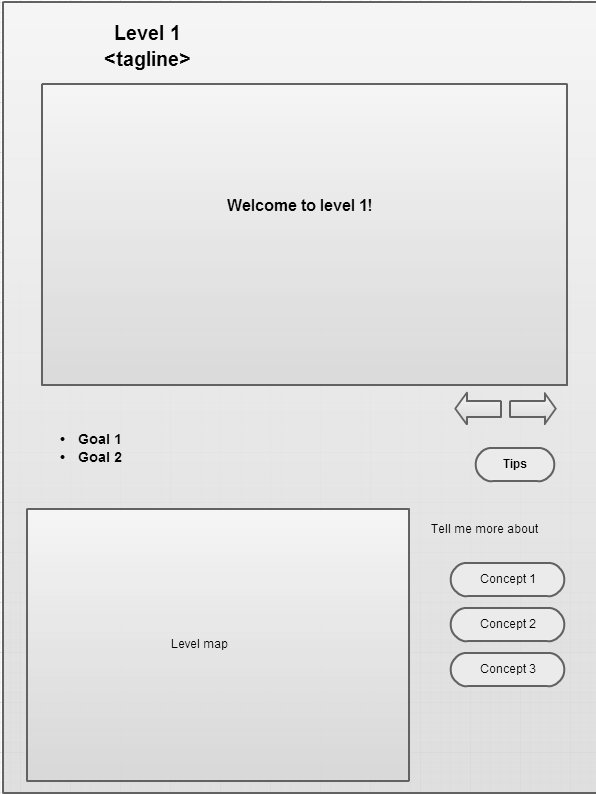
\includegraphics[scale=0.50]{level1_intro_mockup}
	\caption[Introduction window design]{The introduction window design, with the introduction slide show at the top, followed by the goals for this level, a button for tips, the level map, and some buttons for retrieving additional information about the concepts presented.}
	\label{fig:level1_intro_mockup}
\end{figure}

\noindent
Below the slide show, we see a list of the goals for the current level. The goals, together with the level map at the bottom, is the most important information of the level. The level map and the goals are always visible, so that the user has easy access to these when working on the solution for the current level. The level map varies in size, but is always scaled to fit the small frame in the bottom left corner. However, since the player sometimes has to check details of the map, it is possible to make it bigger by clicking on it.

\noindent
Finally, the buttons on the right side of the window represent the \emph{help-on-demand} information that is not visible by default. The \emph{Tips} button provides some tips that are good to know either for solving the current level, or for learning about modeling in general. The hope is that if players get stuck or are unsure about how to proceed, they will see and click this button in an attempt to find help. The \emph{Tell me more about...} buttons provide more detailed information about each concept presented in the current level, available for players who need more information in order to understand the concepts sufficiently, or simply want to learn more.

\subsection{Game Levels}
\label{sec:game_levels}
For the first version of the prototype, only 5 levels were designed and implemented. This was because I wanted to test the prototype with a few users as soon as possible, in order to uncover any serious flaws with the \gls{ui} or the way the introductions were presented as early as possible. 

\noindent
The prototype levels roughly follow the teaching order described in Sect.~\ref{sec:teaching_order}. The first version of the prototype covers steps 1 through 3, with level 5 introducing part of step 4. The game levels are briefly described below.

\subsubsection{Level 1}
Figure~\ref{fig:level1map} displays the map for level 1. The purpose of this level is to introduce the game concept, the main character Malcolm, and the most basic modeling concepts in Reactive Blocks. The goal is pretty much identical to exercise 1 of the tutorial (create a \emph{Hello World!} program), but the game additionally visualizes this task through the game character. The player is provided with the \emph{sayHello} operation, which makes a speech bubble appear next to the character on the level map.

\begin{figure}[htp]
	\centering
	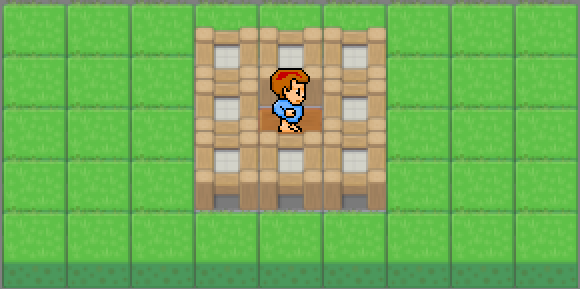
\includegraphics[width=0.6\textwidth]{level1map}
	\caption[Level 1 of the Reactive Blocks game]{Level 1 of the Reactive Blocks game. The player must make the character speak, which makes a speech bubble appear beside him.}
	\label{fig:level1map}
\end{figure}

\noindent
\textbf{Goal:} Make the game character speak the famous words ``Hello world!''

\noindent
\textbf{Concepts introduced:} Activity Steps, Edges, Initial Nodes, Operations, and Activity Final

\noindent
\textbf{Operations:} sayHello

\subsubsection{Level 2}
Figure~\ref{fig:level2map} displays the map for level 2. The purpose of this level is to introduce the player to moving the game character around, and learn about timing delay with \emph{timers}. The goal is to make the character start moving forward, and then add correct timing so that the character will stop moving on top of the star, allowing him to pick it up. The time it takes to move from the starting position to the star is directly proportional to the distance, as it takes 500 milliseconds to cross one tile.

\begin{figure}[htp]
	\centering
	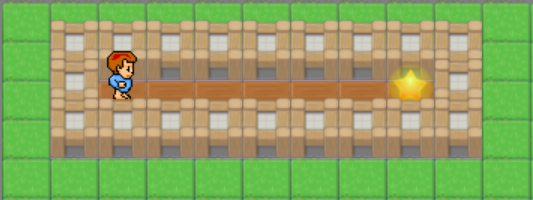
\includegraphics[width=0.7\textwidth]{level2map}
	\caption[Level 2 of the Reactive Blocks game]{Level 2 of the Reactive Blocks game. The player must make the character move 6 tiles forward by timing the movement correctly, and then pick up the star.}
	\label{fig:level2map}
\end{figure}

\noindent
\textbf{Goal:} Make the game character pick up the star

\noindent
\textbf{Concepts introduced:} Moving forward, Timers

\noindent
\textbf{Operations:} moveForward, stop, pickUp

\subsubsection{Level 3}
Figure~\ref{fig:level3map} displays the map for level 3. Modeling wise, this level does not introduce any new concepts, but lets the player become more familiar with timers, and use operations to also change the direction of the game character. Level 3 is a follow-up challenge for level 2.

\begin{figure}[htp]
	\centering
	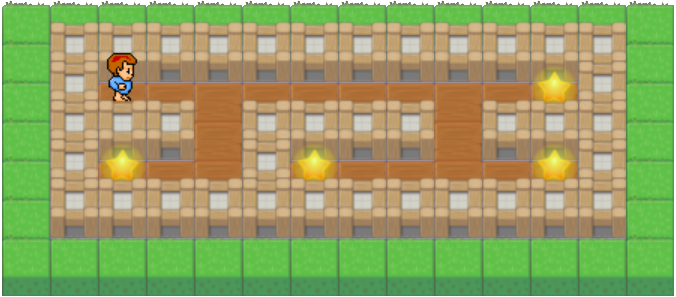
\includegraphics[width=0.8\textwidth]{level3map}
	\caption[Level 3 of the Reactive Blocks game]{Level 3 of the Reactive Blocks game. The player must move the character around the maze, and pick up all the stars.}
	\label{fig:level3map}
\end{figure}

\noindent
\textbf{Goal:} Make the game character pick up all four stars

\noindent
\textbf{Concepts introduced:} Moving in different directions

\noindent
\textbf{Operations:} moveForward, stop, pickUp, turnLeft, turnRight, turnAround

\subsubsection{Level 4}
Figure~\ref{fig:level4map} displays the map for level 4. The purpose of this level is to introduce the player to \emph{decisions}, \emph{alternate branches}, and handling things that may not be known in advance. Players also learn to pass data from operations to decisions, allowing \emph{guards} to be set on outgoing edges.

\begin{figure}[htp]
	\centering
	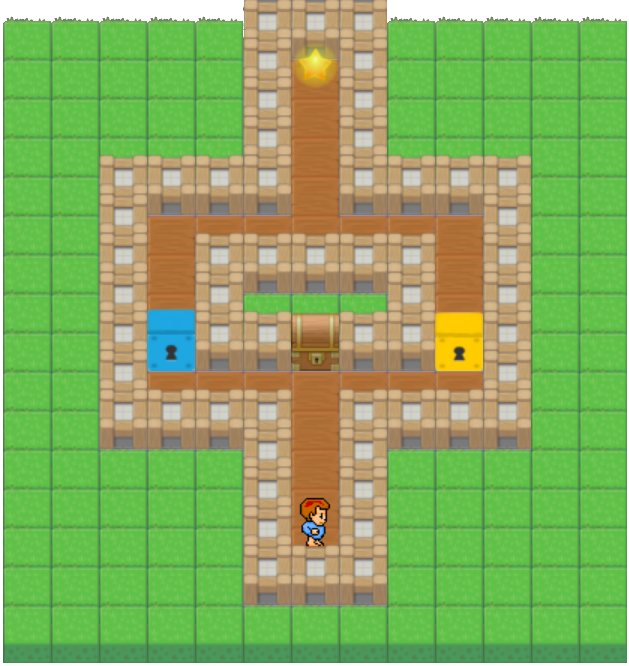
\includegraphics[width=0.7\textwidth]{level4map}
	\caption[Level 4 of the Reactive Blocks game]{Level 4 of the Reactive Blocks game. The player must open the chest to reveal an either blue or yellow key, which allows one lock to be unlocked. The character can then pass through to the star.}
	\label{fig:level4map}
\end{figure}

\noindent
\textbf{Goal:} Open the chest to find a key, unlock the lock matching the key, and pick up the star

\noindent
\textbf{Concepts introduced:} Alternate branches, Decisions, Object flows

\noindent
\textbf{Operations:} moveForward, stop, pickUp, turnLeft, turnRight, turnAround, interact

\subsubsection{Level 5}
With the introduction of alternate branches, activity diagrams can become large and messy. Logic has to be (re)created for each branch, and if more branches follow, we quickly see an explosion of the decision tree. Fortunately, there may be ways of simplifying this, depending on what happens in each branch.

\noindent
Figure~\ref{fig:level5map} displays the map for level 5. There are 4 locks with different colors, meaning that there are 4 possible branches/paths after the chest has been opened. However, the final part of each path is identical, meaning we can use the same sequence to complete the logic. The purpose of this level is to introduce \emph{reuse} to players, by using the same sequence to complete all alternate branches with one or more \emph{merge} nodes.

\begin{figure}[htp]
	\centering
	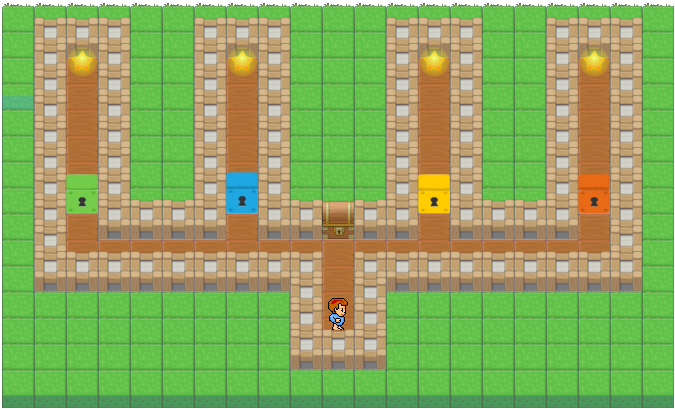
\includegraphics[width=0.8\textwidth]{level5map}
	\caption[Level 5 of the Reactive Blocks game]{Level 5 of the Reactive Blocks game. The player must open the chest to reveal an either green, blue, orange, or yellow key, which allows one lock to be unlocked. The character can then pass through to the star.}
	\label{fig:level5map}
\end{figure}

\noindent
\textbf{Goal:} Open the chest to find a key, unlock the lock matching the key, and pick up the star

\noindent
\textbf{Concepts introduced:} Reuse of sequences, Merge nodes

\noindent
\textbf{Operations:} moveForward, stop, pickUp, turnLeft, turnRight, turnAround, interact

\section{Implementation}
\label{sec:game_implementation}
With the game concept in place, it was time to start working on the prototype implementation. Since Reactive Blocks is Java-based, the natural choice was to start with a Java framework for creating games. I settled for \emph{libGDX},\footnote{\href{http://libgdx.badlogicgames.com/}{LibGDX: Java game development framework (link)}} a Java game development framework licensed under Apache 2.0.\footnote{\href{http://www.apache.org/licenses/LICENSE-2.0.html}{Apache License, Version 2.0 (link)}}

\noindent
Even with a framework as a starting point, implementing the game prototype required considerable work. The game itself was implemented as a JAR to be included with a Reactive Blocks project containing blocks for each level. Graphics are based on or retrieved from various collections of free graphics on the web. For the interested reader, both the full source code\footnote{\href{https://github.com/Desarc/reactive-blocks-tutorials/tree/master/no.ntnu.oyvinric.tutorialgame}{Tutorial Game source code project on GitHub (link)}} and the Reactive Blocks project\footnote{\href{https://github.com/Desarc/tutorial-game}{Tutorial Game release project on GitHub (link)}} is available online.

\noindent
The result is a game prototype with 5 levels, and an introduction part for each level. The level maps were designed using the \emph{Tiled Map Editor}.\footnote{\href{http://www.mapeditor.org/}{Tiled Map Editor website (link)}} Below, each component is described in more detail, using level 4 as an example.

\begin{figure}[htp]
	\centering
	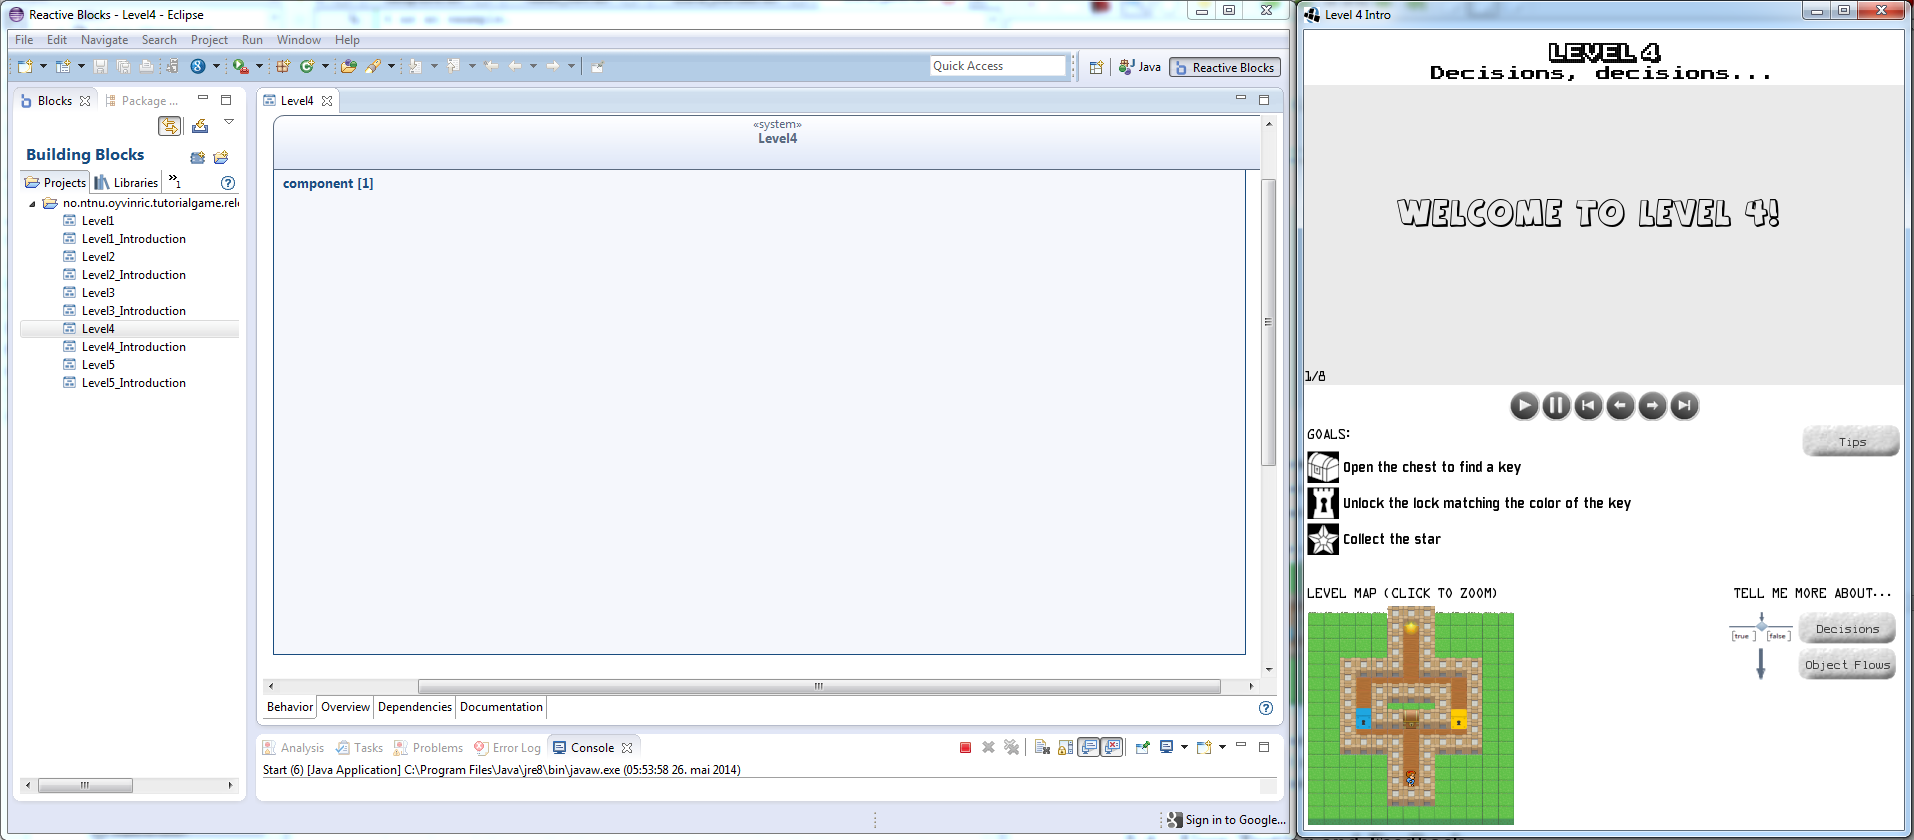
\includegraphics[width=\textwidth]{level4}
	\caption[The Reactive Blocks game user interface]{The Reactive Blocks game interface. On the right side is a regular Eclipse window running the Reactive Blocks perspective with the block for level 4 open. On the right side is the introduction window for level 4.}
	\label{fig:level4}
\end{figure}

\paragraph{The Game Interface}
Figure~\ref{fig:level4} shows the interface of the game on a wide screen (1920x1080 pixels), with the Eclipse window running a Reactive Blocks perspective on the left, and the introduction window on the right. The player starts playing the game by ``building and running'' the \emph{Level1\_Introduction} block, which makes the introduction window pop up. A more detailed view of the introduction window implementation is displayed in Fig.~\ref{fig:level4_intro}. The player can then open the \emph{Level1} block and start modeling, by right-clicking the empty canvas and adding elements. The required operations are already implemented, referencing the JAR with the game logic, and the player can simply add them to the model. An example solution for level 4 is displayed in Fig.~\ref{fig:level4_solution}. When the model is complete, it is time to ``build and run'' the \emph{Level1} block to see if the solution is correct. If this is the case, the player moves on to \emph{Level2\_Introduction} and repeats the process.

\begin{figure}[htp]
	\centering
	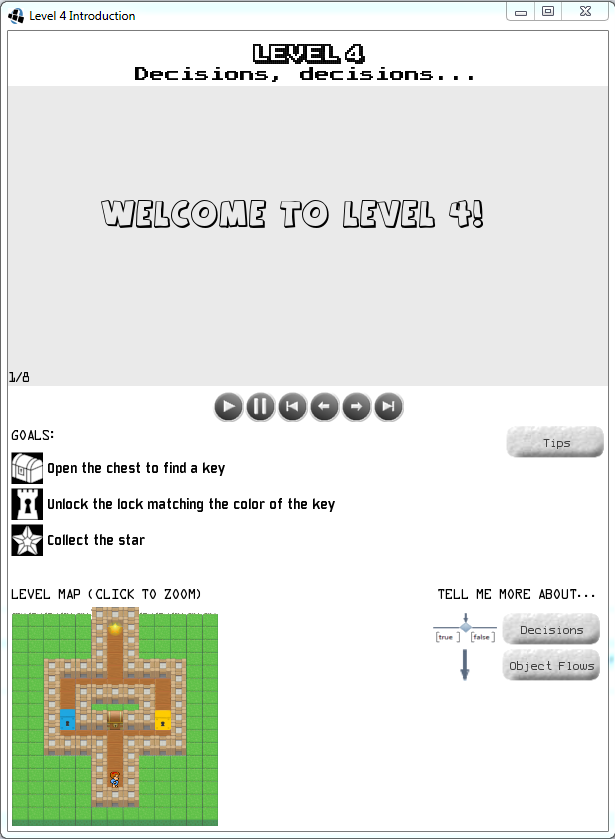
\includegraphics[width=0.85\textwidth]{level4_intro}
	\caption[Reactive Blocks game Level 4 introduction]{The implementation of the introduction window for level 4 of the Reactive Blocks game. This implementation matches the design displayed in Fig.~\ref{fig:level1_intro_mockup}.}
	\label{fig:level4_intro}
\end{figure}

\begin{figure}[htp]
	\centering
	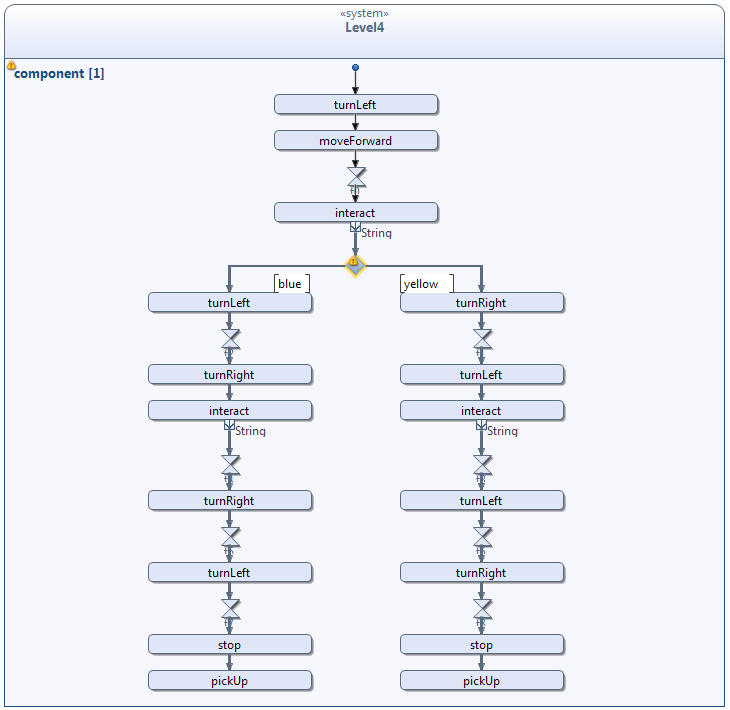
\includegraphics[width=0.8\textwidth]{level4_solution}
	\caption[Reactive Blocks game Level 4 solution]{An example solution for level 4 of the Reactive Blocks game.}
	\label{fig:level4_solution}
\end{figure}

\noindent
The introduction window is described in more detail in Sect.~\ref{sec:game_tutorial}, and matches the design mock-up. Like the rest of the game, it is implemented within the \emph{libGDX} framework. The introduction slide show for each level is available on YouTube.\footnote{\href{http://www.youtube.com/playlist?list=PLoqEHDwb_4oD8LT7n-7Q1dx67HxXwJN_K}{Reactive Blocks Game introductions (YouTube, link)}}

\paragraph{The Game Window}
Figure~\ref{fig:game_window} shows the main game window after level 4 has been completed. This window is opened when the player ``builds and runs'' the \emph{Level4} block after completing the model, and assuming the model is correct, displays the desired behavior of the game character. A short video of a successful run through each level is available on YouTube.\footnote{\href{http://www.youtube.com/playlist?list=PLoqEHDwb_4oA6lkALwIyO7CQx0C4-W57f}{Reactive Blocks Game level completion recordings (YouTube, link)}}

\begin{figure}[htp]
	\centering
	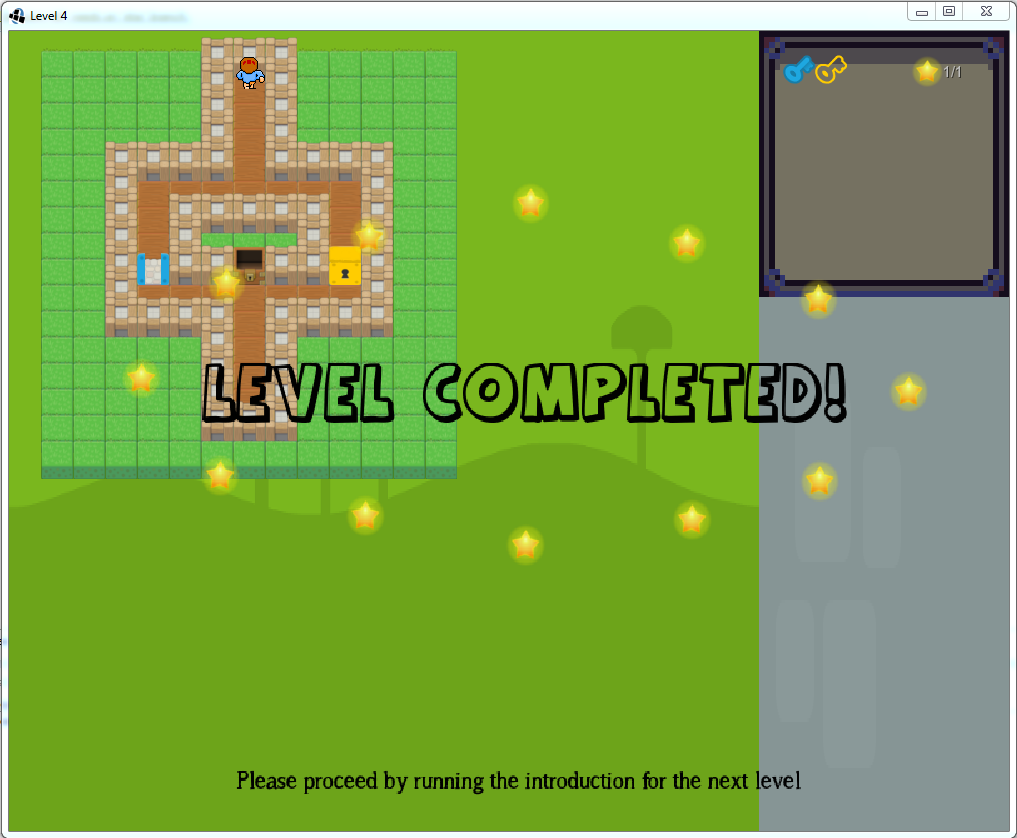
\includegraphics[scale=0.45]{game_window}
	\caption[Reactive Blocks game window]{The game window for the Reactive Blocks game after level 4 has been completed. The level map is displayer on the left, while the right side contains a \gls{hud} informing the user about the current status of the level.}
	\label{fig:game_window}
\end{figure}

\noindent
The main part of the window is the level map, where we can see the game character moving around and interacting with various objects. On the right side is a small \gls{hud}, which displays the current status of the level, such as how many stars have been picked up, how many need to be picked up in total, and which keys have been found.

\section{Usability Testing of the Game}
\label{sec:game_testing}
With a prototype of the game ready, it was time to do some usability testing to see how players are able to work with the \gls{ui}, and grasp the concepts presented sufficiently to complete the levels without help. Suitable test subjects were even harder to come by than with the tutorial in Ch.~\ref{ch:reactive_blocks_tutorial}, but I was able to recruit three volunteers. Two of the test subjects fit within the target audience, having some previous experience with programming and system engineering, while the third subject offers a slightly different perspective, being an experienced gamer.

\noindent
The primary goal for the usability test is to uncover issues about the game that may decrease the quality of the learning experience. Such issues may include poor affordance in the game \gls{ui}, or insufficient, missing, or confusing information about concepts.

\subsection{Testing Method and Collection of Results}
\label{sec:game_testing_method}
The testing session is carried out as a fairly standard discount usability test~\cite{nielsen:discount_usability}, with the significant difference that a functional prototype is used instead of a simple mock-up. The user is presented with some scenarios to go through, in this case starting with instructions on how to set up the game, followed by a challenge to solve for each level. While working on the tasks, the user is encouraged to think aloud in order to give the supervisor (the author) additional information about their choices.

\noindent
Supervisor intervention is kept to a minimum. The supervisor will only intervene when a problem with the game has been clearly established, and there is no point in watching the user struggling further.

\noindent
In an attempt to measure the users' understanding of the concepts presented in each level, the users are asked to fill in a feedback form\footnote{See Appx.~\ref{appx:game_feedback_form}} rating their own understanding of these concepts after the level has been completed. The purpose of the questions in this form is to get an impression on how difficult the game is to understand, if there is anything missing from the introductions, and if the users feel that they have understood the concepts.

\noindent
In accordance with the discount usability test approach, a brief heuristic evaluation of the overall game \gls{ui} is also performed. The \gls{ui} will be evaluated against \emph{The Eight Golden Rules of Interface Design}~\cite{shneiderman:user_interface}.

\subsection{Test Subject 1}
\label{sec:game_testing_subject1}
Test subject 1 is a 25 year old male with a university degree in petroleum engineering. The subject has some previous programming experience with numerical computations in MATLAB or Fortran, but no experience with system engineering. He is however a very experienced player of various video games within different genres.

\noindent
While observing test subject 1 playing the game, I discovered both some problems with the game \gls{ui} and some bugs that needed fixing. I will not go into details about the bugs, but attempt to highlight some of the \gls{ui} issues. Subject 1 spent a total of 83 minutes on the 5 levels of the game.

\noindent
The first thing I noticed was that the subject had trouble following the slide show, which would start automatically and change slide every 10 seconds. It is possible that having a slide show that runs automatically is not a very good idea, considering that users read and understand concepts at different speeds.

\noindent
Throughout the whole game experience, the subject consistently had trouble navigating the Reactive Blocks \gls{ui}, making some tasks unnecessarily difficult to complete, and slowing down the overall progress. This includes things like trouble finding the correct elements, or trying to connect edges to nothing. At one point the subject accidentally double-clicked an operation, bringing up the Java code for the current level, which added some confusion.

\noindent
At level 1, the subject thought that an Activity Final node was required to complete the program. This was a completely logical observation, however unfortunate, since adding an Activity Final node to the application will terminate the game before the user can see that the level is completed. The tip that said an Activity Final node was not needed, was apparently not sufficient, as the subject eventually gave up on understanding what the problem was, and asked for help.

\noindent
In more than one case, the subject was able to complete a level without having correct timing. The game character would just keep walking into a wall until finally the timer expired, and a star was picked up.

\noindent
On level 4, the subject struggled with understanding decisions and guards, particularly which data type should be used. String values \emph{blue} and \emph{yellow} were mentioned in the introduction, but the subject believed the guards should be set to \emph{true} for blue, and \emph{false} for yellow. The subject was also confused by the option of adding an \emph{else} branch from decisions, which was not really necessary in this case. Additionally, it was not clear to the subject where the data would come from, and he started experimenting with \emph{variables}. In the end, the subject needed some help with understanding which data type should be set on the guards.

\noindent
While struggling with level 4, the subject started actively looking for ways to discover what the problem was, and discovered the \emph{analyze} functionality of Reactive Blocks. This could have helped him solve it, but he did not understand the error messages presented.

\noindent
After the subject had understood how to set guards from decisions in level 4, he noticed that the branches could be merged for the final part, which is the learning goal for level 5. Since merge nodes had not yet been introduced, the subject thought the \emph{join} node would be the correct choice, which resulted in some error messages the subject did not understand (in fact, these error messages did not really give any real information).

\noindent
When working on level 5, the subject tried to add multiple outgoing edges from an operation, and set guards on these, without adding a decision node in between. The subject also got confused by the \emph{connector merge} node in Reactive Blocks, as he tried to use this node instead of the regular \emph{merge} node, which he did not discover until later. Finally, the key/lock value corresponding to \emph{red} actually look orange within the game, which added some confusion.

\noindent
Each time the subject would get stuck or have trouble understanding a concept, he would check the tips for that level, or the help-on-demand resources for that concept. The subject needed extra information on levels 1, 4 and 5, but was able to complete 2 and 3 with the information from the introduction alone. Levels 2 and 3 were additionally completed on the first try, while the other levels required some trial and error.

\subsection{Test Subject 2}
\label{sec:game_testing_subject2}
Test subject 2 is a 24 year old male, working on a university degree in Computer Networking and Signal Processing. The subject has some previous programming experience from various university courses, ranging from basic object orientation to microcontroller programming, and some \gls{hci} implementation.

\noindent
Test subject 2's playing session was also far from flawless. Subject 2 encountered many of the same problems with the game as subject 1, in addition to some new issues. Subject 2 actually uncovered more bugs during his session, because his approach to solving the levels touched more edge cases. Subject 2 spent a total of 66 minutes on the 5 levels of the game.

\noindent
First of all, subject 2 struggled with many of the same things related to the Reactive Blocks \gls{ui}. The difference was that subject 2 was familiar with some other software development tools, and thus had some expectations that were not met with the \gls{ui}. However, because of the initial awkwardness and annoyance experienced when working with the Reactive Blocks \gls{ui}, the subject later discovered some actions that would simplify the modeling process on his own, such as duplicating elements or sequences of elements.

\noindent
Subject 2 experienced the same problems in trying to follow the introduction slide show. Sometimes it progressed too fast, and he had to go back to finish previous slides.

\noindent
Like test subject 1, subject 2 also experienced confusion about the \emph{activity final} node. He commented that since the element had been introduced as a way of ``finishing'' a program, it was implied that this element should be the final part of all programs, and was actually \emph{required} to end an activity step.

\noindent
Test subject 2 additionally experienced some confusion about the goals for some levels, such as believing he had to return to the starting point in order to complete.

\noindent
Unlike subject 1, subject 2 was able to better understand decisions and guards, and was thus able to complete levels 4 and 5 more easily. However, since the \emph{object flow} was introduced as an individual concept, he believed this was an element separate from control flow edges, and spent quite some time looking for it.

\noindent
Likely due to his previous programming experience, the subject attempted to use the logical operation \emph{OR} to simplify the alternate branches in level 5. This is unfortunately not possible, as guards in Reactive Blocks only accept \emph{literal} values.

\noindent
Unlike subject 1, subject 2 was able to create the correct logic on his first try for all levels (disregarding the use of \emph{activity final} in level 1). Subject 2 also actively used the \emph{tips} functionality to find help, but rarely needed to check the help-on-demand resources.

\noindent
Subject 2 also mistook the red key/lock pair to be orange.

\subsection{Test Subject 3}
\label{sec:game_testing_subject3}
Test subject 3 is a 24 year old male, with roughly the same background as test subject 2.

\noindent
Like subject 2, subject 3 also uncovered quite a few bugs during his session, also some new ones. Otherwise, the issues encountered were largely the same as with subjects 1 and 2. Subject 3 spent a total of 74 minutes on the 5 levels of the game.

\noindent
Subject 3 began the testing session by commenting right away that he did not prefer the introduction slide show to start automatically, and progress in fixed intervals. The subject would then go on to pause the slide show for each level right away, or go back to the start if he forgot to pause, and then progress manually.

\noindent
With many of the same expectations for the Reactive Blocks \gls{ui} as subject 2, subject 3 also faced the same kind of awkwardness and annoyance when learning to work with it. Having already established that this was an issue, I gave the subject some tips on working with the \gls{ui} in order to lessen his frustration.

\noindent
Like the other two subjects, subject 3 found it natural to include an \emph{activity final} node to complete the program. He also explained that he did not realize the various parts of an activity step were performed without intermediate delay, and thus expected to see the result of completing the level even if the program was terminated (after a delay).

\noindent
Like subject 1, subject 3 was confused about how to add guards to decisions, not realizing he was supposed to first create outgoing edges. He attempted to work around this by using the ``Add else branch'' option in Reactive Blocks, but this proved a more confusing approach, as it created \emph{control flow} edges which may only have \emph{else} guards.

\noindent
Unlike the other subjects, subject 3 preferred to solve some of the levels incrementally, particularly level 3 and 5, by completing part of the logic and checking if everything was correct so far. Subject 3 also spent more time reviewing \emph{tips} and help-on-demand sources than the other subjects. 

\noindent
Subject 3 also attempted the use of the logical operator \emph{OR}, and mistook the red key/lock pair to be orange.

\subsection{Data from the Feedback Forms}
\label{sec:game_feedback_data}
In addition to my observations, each test subject filled in the feedback form included in Appx.~\ref{appx:game_feedback_form}. This section summarizes the data gathered from these forms.

\noindent
The first question asked, for each level, if the introduction part gave enough information to solve that level. All three subjects answered consistently \emph{yes} for all levels, except subject 2 for level 1. Subject 2 further commented that he thought the introduction part gave misleading information about the \emph{activity final} node, causing his solution to level 1 to sort of be both right and wrong at the same time. It was difficult to understand what was going wrong, and subject 2 eventually had to ask for help from the supervisor. As we can see from my observations in the previous sections, this actually also happened with the two other subjects. Since subjects 1 and 3 answered that the introduction part gave them enough despite their trouble, they may have considered this as an oversight of their own, rather than missing information.

\noindent
Question 3 asked the subjects to rate how difficult they found each level to be, and the results are displayed in Tab.~\ref{tab:subject_difficulty}. From the table, we see that all three subjects found levels 2 and 3 to be easier than the others. The two subjects with more diverse programming backgrounds, subject 2 and 3, also consistently experienced each level as being easier than subject 1.

\begin{table}[htp]
	\centering
	\begin{tabulary}{\textwidth}{| C | C | C | C |}
		\hline
		\textbf{Level} & \textbf{Subject 1} & \textbf{Subject 2} & \textbf{Subject 3} \\
		\hline
		1 & Difficult & OK & OK \\
		\hline
		2 & OK & Easy & Easy \\
		\hline
		3 & OK & Easy & Easy \\
		\hline
		4 & Difficult & OK & OK \\
		\hline
		5 & Difficult & Easy & Easy \\
		\hline
	\end{tabulary}
	\caption[Test subject perceived difficulty per level]{The \emph{perceived level of difficulty} for each level and each test subject. Available options were in ascending order \emph{Too Easy}, \emph{Easy}, \emph{OK}, \emph{Difficult}, and \emph{Too Difficult}.}
	\label{tab:subject_difficulty}
\end{table}

\noindent
Question 4 asked the subjects to rate their own level of understanding for each concept presented, and the results are displayed in Tab.~\ref{tab:subject_understanding}. There is a lot of variation, but we should notice that none of the subjects felt they gained a \emph{complete} understanding of \emph{activity steps}, \emph{activity final}, and \emph{timers}. Subjects 1 and 3 actually did not rate their own understanding as complete for any of the concepts presented.

\begin{table}[htp]
	\centering
	\begin{tabulary}{\textwidth}{| C | C | C | C |}
		\hline
		\textbf{Concept} & \textbf{Subject 1} & \textbf{Subject 2} & \textbf{Subject 3} \\
		\hline
		Activity Steps & Partly & Mostly & Mostly\\
		\hline
		Edges & Mostly & Completely & Partly \\
		\hline
		Operations & Mostly & Completely & Mostly \\
		\hline
		Initial Nodes & Mostly & Completely & Mostly \\
		\hline
		Activity Final & Partly & Not at all & Mostly \\
		\hline
		Timers & Mostly & Mostly & Mostly \\
		\hline
		Decisions & Partly & Completely & Mostly \\
		\hline
		Object Flow & Mostly & Completely & Mostly \\
		\hline
		Merge & Mostly & Completely & Mostly \\
		\hline
	\end{tabulary}
	\caption[Test subject self-rated levels of understanding per concept]{The self-rated \emph{level of understanding} for various Reactive Blocks elements by each test subject. Available options were in ascending order \emph{Not at all}, \emph{Partly}, \emph{Mostly}, and \emph{Completely}.}
	\label{tab:subject_understanding}
\end{table}

\noindent
The fifth question asked, for each level, whether the subjects thought they would be able to use the concepts they had just learned about to solve other problems. All three subjects consistently answered \emph{yes} to this question for all levels.

\noindent
In addition to the question asked for each level, there were some final questions. The first question asked whether the subjects \emph{enjoyed} playing the game, to which subjects 1 and 3 answered \emph{yes}, and subject 2 answered \emph{a little}. As a follow up, they were asked to comment on what they did or did not like. While subject 1 left this field empty, subject 2 mentioned that it was a good way of learning concepts, and that it gave him a sense of achievement. Subject 3 mentioned that the \gls{ui} had been somewhat annoying to work it. Finally, the subjects were asked if they would prefer the game as a way to learn about \gls{uml} activities and Reactive Blocks, compared to other options. All three subjects answered in favor of the game.

\subsection{A Side-Note on an Informal Experiment}
\label{sec:game_testing_sidenote}
In addition to the formal usability tests conducted with the three volunteer subjects, I thought it might be interesting to test the game experience on someone completely outside the target audience, just to see what happened. I decided my girlfriend, an elementary school English teacher with no experience even remotely related to programming (she does not like working with computers), would be a suitable subject.

\noindent
The experiment was conducted in an informal way, where she would simply do her best to absorb the information provided in the introductions, and then try to solve the exercises. I helped with some of the parts that were more technical and less relevant, such as preparing Eclipse and Reactive Blocks, and building and running the blocks. If she got completely stuck, I would also offer some hints, primarily about where she could find more information.

\noindent
To my slight surprise, my girlfriend actually handled the problems presented very well. She read the introductions carefully, and easily understood the concepts of operations, tokens and control flow. She handled timers without trouble, struggled a little with decisions (I had to explain what \emph{Strings}, \emph{booleans}, and \emph{integers} were), and used \emph{Merge} nodes perfectly to simplify the logic in level 5. She did spend notably more time on each level than the three subjects in the formal tests (she even got a little more help with \gls{ui} issues), but this could simply be because she was not used to building this particular kind of mental models, added to the fact that she read the instructions extra carefully.

\noindent
Despite her aversion for working with computers and lack of interest for software development, she found the game fun to play because it let her get the sense of mastering a skill she thought was far beyond her abilities. When starting both level 4 and 5, she sighed and exclaimed that \emph{``it looks really difficult!''}, but attacked the problems with determination, reading and re-reading the introductions until things started to make sense.

\noindent
I should also include that while my girlfriend was able to understand the concepts presented sufficiently to solve problems within the context of the game, she admitted to having no idea about how they could be used for other purposes.

\noindent
While I found this experiment to be quite interesting, its informal nature prevents me from drawing any real conclusions. It is likely that a large part of my girlfriend's motivation was to support my thesis work, as opposed to wanting to learn about \gls{uml} activities. Also, despite not having any interest in working with computer-related topics, she could simply be the type of person who has a knack for understanding these things (without even knowing it). All in all, much is left to speculation, but the experiment provides an interesting anecdote for the potential of educational games.

\section{Evaluation of the Tutorial Game}
\label{sec:game_evaluation}
Following the usability test of the game prototype, a formal evaluation of the prototype is prudent. This evaluation is done in three parts, starting with a heuristic evaluation of the game \gls{ui}, followed by a discussion of the usability test result, and finally some suggestions for improvement.

\subsection{Heuristic Evaluation}
\label{sec:game_heuristic_evaluation}
As the first part of evaluating the tutorial game, I conducted a heuristic evaluation of the \gls{ui}. The \gls{ui} primarily consists of three elements, namely the Reactive Blocks modeling environment, the introduction window, and the game window. Since there is little interaction with the game window after it has been opened, this part is discussed in less detail. The Reactive Blocks \gls{ui} is included in the evaluation despite not being designed as a part of this project, because it plays a significant role in the overall usability of the game.

\noindent
The evaluation is performed with respect to \emph{The Eight Golden Rules of Interface Design}~\cite{shneiderman:user_interface}, combined with the context of good practices for games.

\subsubsection{Strive for Consistency}
Similar processes should require similar actions, and elements with similar functions should display similar affordance, making the \gls{ui} feel more consistent for the user.

\noindent
In the introduction window, all buttons for information windows look the same, and perform the same action (though with different content). All these windows may be closed by a corresponding \emph{close} button. Additionally, the buttons for controlling the slide show have similar looks, but different symbols according to their function. The game map displayed in the introduction window is identical to the one found in the game window. The remaining elements are mostly unique, so there are no real inconsistencies.

\noindent
The Reactive Blocks interface is mostly consistent, with a few exceptions. \emph{Edges}, unlike other elements, can not simply be added to the modeling canvas, but must be connected to other elements in both ends. There is no indication of the differing behavior in the \gls{ui}, and the users must discover this on their own. All elements are found in the same menu, and the only thing separating them is a very subtle line. A similar line also separates some other elements in the same, though there is no indication of what the differences between these are.

\subsubsection{Cater to Universal Usability}
The \gls{ui} for the game should be easy to comprehend for any user within the target audience, which may involve detailed explanations for novice users, or useful shortcuts for the more experienced.

\noindent
In the case of the introduction window, this is well-covered. Only the most important information is displayed by default, allowing ``expert'' users to start working on the task right away. Novice users have the option of going through the introduction slide show, viewing tips for the current level, or reading more detailed descriptions of specific concepts.

\noindent
The Reactive Blocks \gls{ui} is likely designed with more advanced users in mind. There are some useful \gls{ui} tools and shortcuts, such as duplicating elements or sequences of elements, but the \gls{ui} is lacking in features for novice users. Most of the possible actions are hidden behind a right-click menu, with no explanations or tooltips. The consequences of this are apparent from the usability test results in Sect.~\ref{sec:game_testing}, where all test subjects struggled with learning the Reactive Blocks \gls{ui}.

\subsubsection{Offer Informative Feedback}
It is important that users understand the consequences of their actions within a given \gls{ui}, and this is highly relevant also for games. Players will want to understand exactly how they can manipulate the game environment in order to overcome challenges and make progress.

\noindent
The introduction window will react to any interaction by changing its content, making the results of any action clear to the user. This includes resizing of the map when it is clicked on, opening sub-windows when clicking buttons, or changing slide when interacting with the slide show controls.

\noindent
For this particular principle, the game window provides some help. When players try to run their model, they will see the result of their logic as movement and actions in the game world. This mapping of created logic to visible result is less obvious within the Reactive Blocks environment, where the only option is to go through activity steps with the \emph{analyze} function.

\noindent
Being a modeling tool, the Reactive Blocks \gls{ui} provides some visual feedback when users are modeling by simply displaying the elements on the canvas. Selecting these elements for manipulation is additionally visualized by highlighting. Building and running a model will generate a project with executable code, and the interface changes to display this project. Some feedback is however less intuitive, such as adding guards to edges. The visual representation of a guard with a \emph{String} value is a small text box, which by default is too small to display the \emph{String}, which is visually replaced by ``[...]''. When creating \emph{else} branches, the visual representation of the guard is often placed in a completely different place on the canvas, such as the upper left corner. Error messages when the user creates invalid models or does something unexpected, are also not always very informative, depending on the user's familiarity with Reactive Blocks and Java.

\subsubsection{Design Dialogs to Yield Closure}
When working with a \gls{ui} involves sequences of actions, they should be organized in a way that makes it clear where the sequence begins and ends. When playing the Reactive Blocks game, most actions are individual, and there are few sequences.

\noindent
In the introduction window, the sequences of actions present consist of no more than two steps. One example is resizing the map, where clicking once makes the map bigger, and clicking again shrinks the map to its original size. The \gls{ui} is then returned to its original state, making it clear that the ``sequence'' has been completed.

\noindent
The Reactive Blocks environment offers a few sequences of actions. One such sequence is building and running the model, which is a sequence of dialog windows the user must go through. After the final window, the environment is changed to display the generated project, indicating that the sequence was successful. There are however sequences of actions that do not yield closure in this way, such as adding edges to the model. When the user selects the \emph{Edge} element, the mouse pointer is changed to an icon indicating edges can be added. Clicking anywhere within the canvas will attempt to add an edge to or from this point, blocking most other actions. After the desired edges have been added, the user must press the \emph{Esc} button in order to clear this functionality and again allow other actions. The user may feel that the sequence has been completed after the edges have been added, when in fact further actions are required.

\noindent
The game window essentially consists of one sequence of actions, with two alternate endings. The player starts the window, and then watches to see if the model was correct. If the model was incorrect, the player will hopefully discover this as a result of what happens in the game world, and simply close the window to continue working on the model. If the model was correct, the player is provided with a message that says ``Level completed!'', indicating that nothing more will happen in the game window. In this case, the user will hopefully also close the window, and then proceed to the next level.

\subsubsection{Prevent Errors}
More important than allowing users to recover from errors, is to prevent users from provoking such errors in the first place. And if errors do appear, they should be possible to recover from, and the \gls{ui} should help the user with this recovery.

\noindent
With the introduction window, provoking errors is virtually impossible. The only interaction available is to click on elements with predefined actions, and these have been thoroughly tested for bugs. The same principle applies to the game window, however bugs are more likely to be present here. Even in the case of errors due to bugs, these should only appear when the player's solution is wrong, causing unexpected behavior, and are thus easily recoverable. Recovery is simply done by closing the game window, fixing the model, rebuilding the system and running again. Of course, this assumes that the player is able to discover the problem after the error has occurred.

\noindent
The Reactive Blocks is a completely different story when it comes to error prevention, likely because it is a relatively young software product, and with vast interaction possibilities. Fortunately, errors are generally recoverable, given that the user understands what is causing the error. For expert users, the error messages provided are generally sufficient, particularly for the cases where models are invalid. In this case, error messages are presented both on-the-fly on the modeling canvas, or summarized in a small window when the user tries to build the model. For novice users however, these error messages may be less informative, since they often assume knowledge of various more advanced concepts. Additionally, there are some error messages that offer no real information at all, such as the one given if the user tries to build a model that is already running.

\subsubsection{Permit Easy Reversal of Actions}
Allowing actions to be undone provides a safety net for the user, encouraging experimentation and speeding up processes.

\noindent
The introduction windows allows easy reversal of any possible action. If the map is zoomed, it can simply be reduced to its original size by clicking on it again. Information windows can be removed simply by closing them, and in the slide show, the user can easily navigate both forwards and backwards at any time.

\noindent
Missing reversal of actions is likely the part about the Reactive Blocks \gls{ui} the test subjects found most annoying (Sect.~\ref{sec:game_testing}). There is no way of easily reversing any action done within the modeling canvas of Reactive Blocks. The user may work around this by for example using the clipboard to temporarily store elements that are to be deleted, or reload any of the ``backups'' Reactive Blocks periodically creates, but neither of these options are good enough for effective use.

\subsubsection{Support Internal Locus of Control}
Users, particularly experienced ones, want to feel in control of the \gls{ui}. This means designing the \gls{ui} in a way that avoids surprises and repetitive, tedious sequences of actions.

\noindent
With the possible actions being quite limited in the introduction and game windows, there is little room for going wrong here. The user can control the slide show, or open additional info windows, neither of which should give the user any surprises.

\noindent
Reactive Blocks fares a little worse here. Always having to go through the right-click menus to add or change elements will likely feel tedious and repetitive to most users, and this was indeed the case for the test subjects in the usability test (Sect.~\ref{sec:game_testing}). Additionally, having to always go through right-click menus could make it difficult for some user to find the information they need, or the right options to produce the result they want.

\subsubsection{Reduce Short-Term Memory Load}
Most users have limited short-term memory, and \glspl{ui} must be designed with this in mind. This includes, among other things, not having to remember information between different screens.

\noindent
The introduction window for the Reactive Blocks game was intentionally made small with this principle in mind. A small window can be placed beside the Reactive Blocks/Eclipse window, meaning the player does not have to remember things like the task or the layout of the map. However, since this is a learning game, some remembering of information is expected. Players have to remember concepts from one level to the next (though it is possible to review previous introductions), and from one slide to the next in the introduction slide show. Additionally, if the player's model is incorrect, it might be necessary to remember what went wrong in order to fix it.

\noindent
Reactive Blocks also does not require users to strain their short-term memory. The model is generally visible on the screen, and in the case of modularization, nested blocks serve as ``black boxes'' with (hopefully) well-defined interfaces. Some memory might be required in the case of operations and knowing what they do, but generally these will have sufficiently descriptive names. Most tasks are relatively simple, and do not require the users to remember long sequences of actions.

\subsubsection{A Summary of Problem Areas}
From the analysis in the previous sections, we see a kind of duality in the adherence to many of the principles. The introduction and game windows present no obvious issues, while the Reactive Blocks modeling environment has quite a few, particularly with respect to consistency, novice user friendliness, reversal of actions, and feedback. The introduction window offers some help with the novice user friendliness part, but it may not be enough.

\noindent
The many issues with the Reactive Blocks \gls{ui} raises the question whether it is the right tool to use in an educational game. Players should not have to spend time learning \gls{ui} quirks that are not necessarily relevant to what they are supposed to learn, or experience frustration with tasks that should be simple and intuitive. This essentially leaves us with two choices: either the Reactive Blocks \gls{ui} must be improved, or the game should be based on a different modeling environment with a more user-friendly interface.

\subsection{Discussion of the Test Results}
\label{sec:game_test_discussion}
The purpose of the usability test (Sect.~\ref{sec:game_testing}) was to uncover in which parts of the game there were issues, and possibly how they could be improved. Both the observations made by the supervisor (the author) during the testing sessions and the feedback forms yielded results that uncovered quite a few issues.

\paragraph{The Reactive Blocks UI} The most prominent issues in the game were related to usability in the Reactive Blocks modeling environment, which caused a lot of frustration. All three test subjects struggled with learning how to work efficiently with the \gls{ui}, and frequently attempted actions that were not possible in the current state. Some of these usability issues are also analyzed in Sect.~\ref{sec:game_heuristic_evaluation}. In short, even with results from only 3 test subjects, we can conclude that the Reactive Blocks \gls{ui} needs some work in order to be good enough for this type of game (this is also supported by the heuristic evaluation).

\paragraph{Activity Final} The test subjects also uncovered some issues with the introductions that will require attention. First of all, it was not clear to any of the users how the \emph{Activity Final} node would affect their programs. Since the game is kind of a special case, all 3 subjects made the ``mistake'' of adding this node at the end of their logic. Players likely need clearer information about what the \emph{Activity Final} node does, and why the game is a special case with regard to this.

\paragraph{Automatic Slide Show} Having an side show that starts automatically, and then changes slide after a fixed delay, might be a bad idea. People read and understand at different speeds, and will probably prefer to control the slide show themselves. All 3 test subjects had to either pause the slide show or go back one or more steps, because it progressed too fast.

\paragraph{Incorrect Timing} In several cases, the test subjects were able to complete a level despite having set the timers to wrong values. This could be interpreted as a kind of ``cheating by laziness'', and should be considered a potential problem. If found to be disruptive of the learning experience, punishing wrong timing by not allowing the level to be completed could be an option.

\paragraph{Decisions and Guards} All 3 test subjects had some trouble figuring out how to work with decisions and guards, some more than other. The main issues involved figuring out how and where to place the various elements, such as understanding that guards had to be set on the outgoing edges from decisions. Additionally, there was confusion about data types, and what the values of the guards should be. This is actually something that touches programming a little bit more than modeling, but it is a part of working with Reactive Blocks, and thus needs to be made clear to the player in some way.

\paragraph{Tips and Help-on-demand} These resources were available for the purpose of helping players figure out how to proceed if they got stuck. All 3 test subjects ended up reviewing either the tips or the help-on-demand resources at some point, because they were unsure how to proceed. These resources were successful in the sense of being discoverable and available when the test subjects got stuck, but it is unclear whether they provided the information the test subjects were looking for.

\paragraph{Expert User Limitations} Test subjects 2 and 3 both attempted to use the logical operator \emph{OR} in guards. This is likely a result of the test subject being more advanced users in the realm of programming and software development, and thus found this to be a natural solution. This is not necessarily a problem, since more advanced users are more likely to quickly figure out what works and what does not.

\paragraph{Incremental Problem Solving} While test subjects 1 and 2 preferred to complete their logic before getting visual feedback from the game, test subject 3 chose to implement part of the logic, and then get feedback on the correctness of the logic so far. This shows that the game allows multiple problem solving strategies, accommodating different types of players.

\paragraph{Colors} All 3 test subjects mistook the red key/lock pair in level 5 to be orange (even the author has to agree that it does in fact look orange). Such inconsistencies inadvertently make the game more difficult, as players may spend time trying to fix mistakes they think are caused by something else.

\paragraph{Difficulty Level} The answers from the feedback forms indicate that the difficulty of the levels varies. More specifically, levels 2 and 3 may be easier for most players to understand and complete than levels 1, 4, and 5. It is inevitable that for many players, some levels will be more difficult than others, since some concepts will be more difficult to understand, and this is not a problem, so long as the level does not become \emph{too} difficult. The test subjects also experienced the difficulty levels to be different, but the fact that none of them rated any of the levels as \emph{too difficult} or \emph{too easy} is taken as a good sign.

\paragraph{Information in Introductions} Apart from the previously mentioned issues with the introductions, there seem to be no significant pieces of information missing, and no information present that is redundant or irrelevant. All 3 test subjects actively used the introduction parts to complete the levels, and found these to be useful overall.

\paragraph{Complete Understanding} From the results of the feedback forms, we can observe that two of the test subjects did not feel that they gained \emph{complete} understanding of any of the concepts presented. Additionally, there were some concepts that not even the last test subject gained complete understanding of. This is certainly undesirable, as we want players to learn these concepts thoroughly, though within the realms of what is actually possible with just a short game.

\paragraph{Enjoyment} Finally, we should observe that none of the test subjects answered that they did \emph{not} enjoy the game. They collectively thought the game would be the preferred way of learning about \gls{uml} activities and Reactive Blocks. The game appears to do a good job of providing learners with an immersive experience and a sense of achievement.

\subsection{Fulfillment of Goals}
\label{sec:game_goal_fulfillment}
Section~\ref{sec:game_goals} listed some goals that were set in advance for the game. With a prototype in place, it is prudent to review the goals, and see whether they have been met, or if any require more attention. It is also taken into consideration that we are only working with a \emph{prototype} that is not yet complete.

\noindent
The game certainly provides a sort of immersive learning experience for players, allowing them to learn concepts and solve problems within the game environment. The immersion is however slightly impaired by the game environment being distributed over different platforms, with the introductions, game world and modeling environment being separate entities. This is also unlikely to change as prototype development continues, since we are dependent on the Reactive Blocks environment. This goal is thus considered to be only partially fulfilled, with potential for improvement.

\noindent
Players are given freedom in the game by being able to use any available elements to find their own solutions, and they can also choose how much information they want to absorb before starting on the tasks. There are hardly any limits to the players' freedom, however. Players are guided through a ``learning path'' where they are introduced to only a few concepts at a time, limiting the amount of information they need to process at a given time. However, the entire Reactive Blocks modeling environment is available to the players, even though many parts of it are less relevant, especially for the first levels. This may add some confusion and complexity to the learning experience, which may slow down progress for a some users. This goal is then also only partially fulfilled, as there could be additional advantages gained from providing a more limited modeling environment, and is also unlikely to change as development continues.

\noindent
All test subjects (even in the informal test) were able to get started on solving level 1 relatively quick. At the same time, the test subjects had different impressions of the difficulty of various levels. The current levels are still likely too easy to really be challenging for more experienced users, but this can be taken into consideration as development continues. In addition to adding more concepts, we can design additional challenge levels for each concept that require deeper understanding.

\noindent
A lot of the issues from the tutorial in Ch.~\ref{ch:reactive_blocks_tutorial} were unfortunately still present in the game. These were mainly issues related to Reactive Blocks, such as no real limits on freedom, insufficient visual mapping of \gls{ui} elements, and exposure to quite a few complexities and processes that were less relevant to the players at their current experience level. Some additional efforts were made to help players find the correct \gls{ui} elements in Reactive Blocks, but test subjects still had trouble with some parts, particularly decisions. It was also still not possible to really have everything in one place, but this was significantly improved from the tutorial, with the introduction window. The one goal that was really improved from the tutorial was to offer help-on-demand resources, which was done in the form of tips for each levels, and additional information pages for each concept. These were used to various degrees by the test subjects when they got stuck on something.

\noindent
It is clear that there is still a long way to go before all these goals can be met, and we potentially have an \emph{excellent} learning tool (as opposed to only a \emph{good} one). The primary obstacle appears to be the Reactive Blocks environment, and the limitations it poses on implementing several of these goals. Currently, the game itself is actually developed completely independent of Reactive Blocks, which is simply used to control it though an \gls{api}. This means that it would be trivial to change to a different modeling environment. The challenge in this is that there are few options available, and creating a \gls{uml} activity modeling framework from scratch would require considerable effort.

\subsection{Suggestions for Improvement}
\label{sec:game_improvement}
The current version of the prototype serves as a pretty good starting point for a \gls{uml} activity learning game, but there are still some things that can, and should, be improved.

\paragraph{Better Modeling Environment} The Reactive Blocks modeling environment seems to currently be the greatest obstacle for improving the game experience. One option is to modify the modeling environment in the context of the game, so that it provides users, particularly novices, with a smoother learning experience. This requires the Reactive Blocks development team to implement this, which is unlikely to happen any time soon, since they likely have other priorities. The other option is to use a different modeling environment, for example one created specifically for the purpose of being used with the game. The feasibility of the latter option is however unclear, as implementing a \gls{uml} activity modeling framework is no trivial task.

\paragraph{Refining of Introductions} The usability test uncovered some issues with the introduction part that should be improved, such as confusion about the \emph{Activity Final} node. The introductions need to be refined with these specific issues in mind, without inadvertently introducing other issues. Additionally, introduction parts for additional levels within the game should not only be carefully designed, but thoroughly tested to verify that they provide the information required in a clear and simple way.

\paragraph{More Levels} Since this is only a first prototype, it only covers part of the \gls{uml} activity topic, with many concepts left untouched. The prototype should be extended with more levels that introduce players to all of these concepts, and possibly also with levels that add additional challenges allowing deeper understanding to some of the concepts.

\noindent
Some level ideas to introduce additional concepts follow:
\begin{itemize}
	\item{\textbf{Concurrency and Forks:}} Add more characters to the game, allowing the player to control several characters simultaneously.
	\item{\textbf{Events:}} Instead having to perfectly time cooperation between several game characters, make interaction operations send \emph{events} that other characters can listen for.
	\item{\textbf{Joins:}} Similar to events, levels can be designed so that the player will benefit from synchronizing actions between multiple game characters with the join node.
	\item{\textbf{Modularization:}} Design the level so that the same actions are repeated in several places. The player can then create an ``action module'' in the form of a \emph{local block} that can be reused in several places.
\end{itemize}

\paragraph{Minor Fixes} In addition to these three major points, I compiled a long list of minor fixes following the testing sessions. These will not be listed here, but include things like bug fixes, not starting the slide show automatically, and changing the color of the red key/lock pair to orange.

\noindent
Unfortunately, limitations on time prevent me from continuing the development of the prototype or conducting additional tests within the scope of this project. However, a faculty representative at ITEM, \gls{ntnu} has expressed some interest in using the game as an introduction to the world of software for first-year students later this year, so I will eventually make some adjustments to prepare the game for this purpose, in case it becomes relevant.
